%------------------------------------------------------------------------------
%
%	dailytax.tex
%
%	This document is written around daily taxation idea which allows to
%	simplify significantly sosial security law sections. Daily tax also
%	makes possible to have negative daily tax values supporting peoples
%	doing unsecure work with so called zero agreement, which means that
%	they have work from 0 to 40 hours in week. While digitalization
%	proceeds further and purchasing comes much more faster and effective
%	some peoples have problems to manage they consumption so that unsecure
%	monthly money may easily run out causing problems. Daily taxation can
%	help by quaranteeing that every day peoples account have some even
%	small amount of money available. It makes peopes life much secure and
%	eases stress from life security even if monay amounts are not any
%	bigger than today.
%
%	AUTHOR: Ari Potkonen /JARVENPAA/ Mon Jun 28 2022
%
%	LICENSE:	All referred trademarks, logos and brand names are the
%			property of their respective owners. This document is
%			licensed under CC-BY-SA licensing scheme.
%
%			Any of the trademarks, service marks, collective marks,
%			design rights, or similar rights that are mentioned,
%			used, or cited are the property of their respective
%			owners. Their use here does not imply that you may use
%			them for any purpose other than for the same or a
%			similar informational use as contemplated by the
%			original author of document licensed under the CC-BY-SA
%			licensing scheme. Author cannot grant any rights to use
%			any otherwise protected materials. Your use of any such
%			or similar incorporeal property is at your own risk.
%
%	LANGUAGE:	LaTeX2e to be used with latexmk
%
%
%	REFERENCE (http://latex-project.org/help/books , http://tug.org/books):
%
%	- http://ctan.org/starter
%	  http://ctan.org/pkg/amsmath
%	  http://ctan.org/pkg/biblatex
%
%	- http://wikibooks.org/wiki/LaTeX
%	- http://wikipedia.org/wiki/BibTeX
%	- http://bibtex.com/format/fields
%	- http://loc.gov/marc
%	- http://issn.org
%
%	- Michel Coossens, Frank Mittelbach, Alexander Samarin:
%	  The LaTeX Companion, Addison-Wesley Company, Inc.
%	  United States of America 1994.
%
%	- Norman Walsh:
%	  Making TeX Work, O'Reilly & Associates, Inc.
%	  United States of America 1994.
%
%	- https://archive.org/details/B-001-002-139
%	  https://archive.org/items/B-001-002-139/Donald_Knuth_-_The_Tex_Book.pdf
%	  https://ctan.org/tex-archive/systems/knuth/dist/tex/texbook.tex
%	  https://visualmatheditor.equatheque.net/doc/texbook.pdf
%
%	- https://www.texlive.info/CTAN/info/impatient/book.pdf
%
%
%	Edition defines major releases of document.	
%
%	EDITION:	0
%
%	Version defines minor changes which can be brought available online.
%
%	VERSION:	
%
%	CHANGED:
%	DOCUMENT HISTORY:
%
%	FUTURE:
%
%	COMPILE:	make
%			make clean
%
%------------------------------------------------------------------------------
%         1         2         3         4         5         6         7
%123456789012345678901234567890123456789012345678901234567890123456789012345678
%-DOCUMENT PREAMBLE------------------------------------------------------------
% http://wikipedia.org/wiki/Ebook
% http://ctan.org/pkg/ebook
% http://ctan.org/pkg/fontspec
% http://www.linux.fi/wiki/LaTeX
% file:///usr/share/doc/texlive-doc/generic/knuth-pdf/index.html
% http://wikipedia.org/wiki/TeX
% http://wikipedia.org/wiki/LaTeX % /usr/share/doc/texlive-doc/latex
% http://wikipedia.org/wiki/XeTeX % xetex/xetexref/xetex-reference.pdf
% http://wikipedia.org/wiki/LuaTeX % doc/texlive-doc/luatex/base/luatex.pdf
% http://wikibooks.org/wiki/LaTeX/Fonts
% http://users.jyu.fi/~lehtonen/texopas/
% http://tug.org/texlive/mapenc.html
% http://tug.org/texinfohtml/kpathsea.html#Debugging
% http://tug.org/pracjourn/2012-1/luca/luca.pdf
% http://wikibooks.org/wiki/LaTeX/Document_Structure
% http://wikipedia.org/wiki/LuaTeX http://luatex.org
% http://kdp.amazon.com/en_US/help/topic/G201834180#trim
% http://github.com/psampaz/latex-nonfiction-ebook-template-1
% http://mirrors.ctan.org/macros/latex/contrib/a4wide/a4wide.pdf
% http://github.com/jfogarty/latex-nonfiction-ebook-template/blob/master/eBook.tex
% http://raippa.fi/matem/JohdatusLaTeXiin/Tyokalut/086%20Suomen%20kielen%20tuki
% /usr/share/doc/texlive-doc/latex/comprehensive/symbols-a4.pdf
% /usr/share/doc/texlive-doc/plain/impatient/book.pdf
% http://ctan.org/topic/class article proc minimal report book slides memoir letter
% [ebook,oneside,openany] 
%\documentclass[12pt,a4paper,finnish,oneside]{article}
%\documentclass[11pt,twoside,openright]{book}
%\documentclass[a4paper,finnish]{report}
%\documentclass[a5paper,draft]{memoir} % texlive-doc/latex/memoir/setpage-example.pdf
\documentclass[a5paper,final]{memoir} % texlive-doc/latex/memoir/memman.pdf
%\documentclass[10pt,a5paper]{book}
%\documentclass[a4paper]{report}
%\documentclass[a4paper]{book}
%\documentclass[a5paper]{book}
%\usepackage{geometry} % /usr/share/doc/texlive-doc/latex/geometry/geometry.pdf
%\usepackege[size=pocket. bleed=false, color=false]{createspace}
%\usepackage{ebook}
%\usepackage{times}
%\usepackage[cp850]{inputenc} % DOS
%\usepackage[ansinew]{inputenc} % Windows
%\usepackage[utf8]{inputenc} % Linux, UTF-8
%\usepackage[utf8x]{inputenc} % Linux, UTF-8
%\usepackage[latin1]{inputenc} % Linux
%\usepackage[LGR,T1,OT1]{fontenc} % /usr/share/doc/texlive-doc/latex/base/encguide.pdf
%\usepackage[english,finnish]{babel} % \selectlanguage{finnish}
%\usepackage[finnish]{babel} % /usr/share/doc/texlive-doc/latex/babel/babel.pdf
\usepackage[english]{babel} % /usr/share/doc/texlive-doc/latex/babel/babel.pdf
\usepackage{advdate} % /usr/share/doc/texlive-doc/latex/advdate/advdate.pdf
\usepackage{mathtools}
\usepackage{fontspec} % /usr/share/doc/texlive-doc/latex/fontspec/fontspec.pdf
%\usepackage{fontsetup} %
% cm, cm-unicode unicode
%\usepackage{xunicode} % for XeLaTeX only xelatex/xecjk/xunicode-symbols.pdf
\usepackage[gen]{eurosym} % doc/texlive-doc/fonts/eurosym/testeuro.pdf
%\usepackage{icomma} % desimalcomma doc/texlive-doc/latex/was/icomma.pdf
%\usepackage{textualicomma} % latex/textualicomma/textualicomma-doc.pdf
%\usepackage{marvosym} % doc/texlive-doc/fonts/marvosym/marvosym-doc.pdf
%\usepackage{beton} % /usr/share/doc/texlive-doc/latex/beton/beton.pdf
%\usepackage{euler} % /usr/share/doc/texlive-doc/latex/euler/euler.pdf
%\usepackage{eulervm} % /usr/share/doc/texlive-doc/latex/eulervm/eulervm.pdf
%\usepackage{fourier} % doc/texlive-doc/fonts/fourier/fourier-doc-en.pdf
%\usepackage{concmath} % /usr/share/doc/texlive-doc/fonts/concmath/concmath.pdf
%\usepackage{amsthm} 
%\usepackage{amsbsy}
%\usepackage{amstex} % /usr/share/doc/texlive-doc/amstex/base/amsguide.pdf
%\usepackage{amsmath} % /usr/share/doc/texlive-doc/latex/amsmath/amsmath.pdf
%\usepackage{amssymb} % /usr/share/doc/texlive-doc/fonts/amsfonts/amssymb.pdf
%\usepackage{amsfonts}
%\usepackage{mathalfa}
%\usepackage{mathspazo} % doc/texlive-doc/latex/mathpazo/pazotest.pdf
%\usepackage{mathdesign} % doc/texlive-doc/fonts/mathdesign/mathdesign-doc.pdf
%\RequirePackage{unicode-math} % texlive-doc/latex/unicode-math/unicode-math.pdf
\usepackage{unicode-math} % doc/texlive-doc/latex/unicode-math/unicode-math.pdf
%\usepackage{notomath} % doc/texlive-doc/fonts/notomath/notomath-doc.pdf
%\usepackage{newtxtext,newtxmath} % http://ctan.org/pkg/newtx
%\usepackage{newpxtext,newpxmath} % http://ctan.org/pkg/newpx
%\usepackage{textcomp} % http://ctan.org/pkg/textcomp

%find /usr/share/texlive -type f -iname "*math*.sty"
%/usr/share/doc/texlive-doc/latex/fontspec/fontspec.pdf
%/usr/share/texlive/texmf-dist/fonts/TYPE/MODE/SUPPLIER/TYPEFACE/dpiNNN/
% http://gnu.org/software/freefont
% http://savannah.gnu.org/projects/unifont
% /usr/share/texlive/texmf-dist/fonts/opentype/public/gnu-freefont
% /usr/share/texlive/texmf-dist/fonts/truetype/public/gnu-freefont
% GNU Fonts with font exception http://gnu.org/licenses/gpl-faq.html#FontException
% fc-list :foundry=psbk:fontformat=CFF family
%  Junicode http://wikipedia.org/wiki/Junicode
%	Junicode Two Beta
% fc-list :lang=en family | grep Linux
%  Linux Libertine http://wikipedia.org/wiki/Linux_Libertine
%	Linux Biolinum O
%	Linux Libertine O
%\setmainfont{Linux Biolinum O}
\setmainfont{Linux Libertine O}
% fc-list :foundry=GNU :fontformat=TrueType family
%  GNU FreeFont http://wikipedia.org/wiki/GNU_FreeFont
%  GNU Unifont http://wikipedia.org/wiki/GNU_Unifont
%	FreeSerif
%	FreeSans
%	FreeMono
%	Unifont
%\setmainfont{FreeSerif}
%\setmainfont{FreeSans}
%\setmonofont{FreeMono}
%\setmainfont{Unifont}

% SIL Open Font License https://openfontlicense.org
% fc-list :foundry=GOOG:fontformat=CFF family | sort -u
%  Noto http://wikipedia.org/wiki/Noto_fonts
%	Noto Mono
%	Noto Sans
%	Noto Serif
% fc-list :foundry=SIL :fontformat=CFF family
%  Gentium http://wikipedia.org/wiki/Gentium
%	Gentium
%\setmainfont{Noto Sans}
%\setmainfont{Noto Serif}
%\setmonofont{Noto Mono}
%\setmathfont{notomath}
%\setmainfont{Gentium}

%\usepackage{nicefrac}
%\usepackage{xfrac} % doc/texlive-doc/latex/l3packages/xfrac/xfrac.pdf
%\usepackage{fp} % /usr/share/doc/texlive-doc/latex/fp/documentation.pdf
%\usepackage{xfp} % /usr/share/doc/texlive-doc/latex/l3packages/xfp/xfp.pdf
%\usepackage{tikz} % /usr/share/doc/texlive-doc/generic/pgf/pgfmanual.pdf
%\usetikzlibrary{calc}
%\usepackage{calc} % /usr/share/doc/texlive-doc/latex/tools/calc.pdf
%\usepackage{calculation} % /texlive-doc/latex/calculation/calculation.pdf
%\usepackage{calculator} % doc/texlive-doc/latex/calculator/calculator.pdf
%\usepackage{sagetex} % /usr/share/texmf/doc/latex/sagetex/sagetex.pdf
%\usepackage{fig}
%\usepackage{righttag}
%\usepackage{epic}
%\usepackage{eepic}
%\usepackage{dyntree} % /usr/share/doc/texlive-doc/latex/dyntree/dyntree.pdf
%\usepackage{pst-tree} % doc/texlive-doc/generic/pst-tree/pst-tree-doc.pdf
%\usepackage{pst-jtree} % doc/texlive-doc/generic/pst-jtree/pst-jtree-doc.pdf
%\usepackage{pst-qtree} % texlive-doc/generic/pst-qtree/pst-qtree-manual.pdf
%\usepackage{synttree} % doc/texlive-doc/latex/synttree/synttree.pdf
%\usepackage{ecltree} % doc/texlive-doc/latex/ecltree/ecltreesample.pdf
%\usepackage{xytree} % doc/texlive-doc/latex/xytree/xytree-doc-en.pdf
%\usepackage{float} % /usr/share/doc/texlive-doc/latex/float/float.pdf
%\usepackage{graphicx} % doc/texlive-doc/latex/graphics/graphicx.pdf
%\usepackage{svg} % /usr/share/doc/texlive-doc/latex/svg/svg.pdf
%\usepackage{svg-extract} 
\usepackage{epsfig} % /usr/share/doc/texlive-doc/latex/graphics/epsfig.pdf
\usepackage{rotating} % share/doc/texlive-doc/latex/graphics/rotating.pdf
%\usepackage{figlatex} % doc/texlive-doc/support/latex-make/figlatex.pdf
%\usepackage{pictex}
%\usepackage{picture} % /usr/share/doc/texlive-doc/latex/picture/picture.pdf
%\usepackage{showidx}
%\usepackage{trees}
%\usepackage{siunitx} % /usr/share/doc/texlive-doc/latex/siunitx/siunitx.pdf
%\usepackage{gensymb} % /usr/share/doc/texlive-doc/latex/gensymb/gensymb.pdf
%\usepackage{textcomp} % 
\usepackage{supertabular} % texlive-doc/latex/supertabular/supertabular.pdf
%\usepackage{verbatim} % /usr/share/doc/texlive-doc/latex/tools/verbatim.pdf
%\usepackage{lscape} % /usr/share/doc/texlive-doc/latex/graphics/lscape.pdf
%\usepackage{pdflscape} % doc/texlive-doc/latex/pdflscape/pdflscape.pdf
\usepackage{csquotes} % doc/texlive-doc/latex/csquotes/csquotes.pdf
%\usepackage{bibtopic} % doc/texlive-doc/latex/bibtopic/bibtopic.pdf
%\usepackage{babelbib} % doc/texlive-doc/bibtex/babelbib/babelbib.pdf
%\usepackage[backend=bibtex,defernumbers=true,sorting=nty]{biblatex}%
%\usepackage[backend=biber,babel=other]{biblatex} % /usr/share/texmf/doc/bibtex/biber/biber.pdf
%\usepackage[backend=biber,autolang=other]{biblatex} % doc/texlive-doc/bibtex/biber-ms/biber-ms.pdf
\usepackage{biblatex} % /usr/share/doc/texlive-doc/latex/biblatex/biblatex.pdf
%\usepackage{url} % /usr/share/doc/texlive-doc/latex/url/url.pdf
%\usepackage[hyphens]{url} %  \PassOptionsToPackage{hyphens}{url}
%\PassOptionsToPackage{hyphens}{url}
\usepackage{xurl} % doc/texlive-doc/latex/xurl/xurl.pdf Penalties for biblatex
\usepackage[hidelinks]{hyperref} % texlive-doc/latex/hyperref/hyperref-doc.pdf
%\usepackage[bookmarks=true,hidelinks]{hyperref} % hyperref/hyperref-doc.pdf
\usepackage{bookmark} % /bookmark/bookmark.pdf Redefine hyperref’s bookmarks.
\usepackage{breakurl} % /usr/share/doc/texlive-doc/latex/breakurl/breakurl.pdf
%\addbibresource{biblatex.bib}
\bibliography{biblatex}
%\usepackage[nottoc,numbib]{tocbibind}
\usepackage{makeidx} % /usr/share/doc/texlive-doc/latex/imakeidx/imakeidx.pdf
\makeindex
%-DOCUMENT PREAMBLE END--------------------------------------------------------
\begin{document}
%\pagestyle{plain}
%-DOCUMENT FRAME --------------------------------------------------------------
%-TITLE PAGE-------------------------------------------------------------------
%\clearpage
%\begin{titlepage}
\pagenumbering{gobble}
%\pagestyle{empty}
\title{\Huge\textbf{Daily Tax} \linebreak DRAFT \linebreak \linebreak
%
\includegraphics[height=64pt,width=64pt]{figures/dtaxlogo.eps}}

\includegraphics[height=64pt,width=64pt]{figures/dtaxlobw.eps}}
%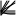
\includegraphics[height=64pt,width=64pt]{figures/dtaxlotb.eps}}
\author{\Large Potkonen Ari} 
%\SetDate[31/08/2023]
\maketitle
%\end{titlepage}
\pagebreak
%-PREFACE----------------------------------------------------------------------
%\pagebreak%\clearpage
\pagestyle{plain}
\parindent 0pt
%\frontmatter
\setcounter{page}{1}
\pagenumbering{roman}
%------------------------------------------------------------------------------
%
%	preface.tex Document preface part
%
%	INCLUDE FILE FOR LaTeX2e DOCUMENT
%
%	AUTHOR: Ari Potkonen /JARVENPAA/ Mon Jun 28 2022
%------------------------------------------------------------------------------
%         1         2         3         4         5         6         7
%123456789012345678901234567890123456789012345678901234567890123456789012345678
%-BEGIN OF INCLUDE FILE--------------------------------------------------------
%\chapter{Preface}
PREFACE
%\addcontentsline{toc}{chapter}{Preface}
%\index{preface}
\label{preface}

\vskip\baselineskip
As I have been quite long time Finnish citizen I have been seeing later
development, what it does when preemptive support for peoples, families and
children's heath, education and social care has been reduced year by year.
Now lot of money goes to care serious results from this habit and grown
average age. Worst thing here is that caring problems and re-enabling
preemptive care with current system and existing maintenance ratio goes over
budget if nothing else is done. And many peoples own budget has already failed
partly because we as society has been allowed to sell out and therefore from
local monopoles for electric delivery and significantly determinative market
positions on rentable property, housing and apartments market. Besides these
there are IT and goods logistic costs having external cream pealers groups on
significant market position. These areas are used to squeez money out from our
society, it's partly increased peoples support need, and this has been led to
higher support during the years, support which is now teared down. Problem is
that peoples are now left between profitmakers demands and subventions closing
sosiety created realities. We could already say that shit has hit into fan.
% and smell lingers around badly.
Overloaded, less paid healthcare workers are already escaping from profession
area\cite{KEVA_tyovoimaennuste}, medical institutions see declining amount of
applicants to profession area courses\cite{YLE202209221026}.
Teachers comment seriously that if knew current situation on work market when
started studies did not choosed to become a teacher. Etc.

\vskip\baselineskip
How we came to this situation at 2023 ?
\vskip\baselineskip
When looking national law making which does basement for Finnish wellbeing
society we need to note one bad habit we have. To maintain wellbeing society
new laws are nearly always made as small tweaks to existing law by adding new
law section, new on/off-rule or rules. After years of this kind of operation
the result is awful for normal citizens. It is mess of "on/off, on/off, if
then else on/off,..." -rules. It's nightmare for people having scarce
resources and need for help. Especially people lacking good digital
information search, bookkeeping and management capabilities is in really deep
shit! Fin\-nish nation has help-begging system for pen, paper and physical
access -peoples, and for others\cite{StudentHousingAllowance}, it's resource
consuming and inhumane. You are really pushed down before you can get
anything, if even then\cite{KELA_BASIC_ASSISTANCE_HalfOrNone}. Finnish mental
health and suicide statistics tell the truth\cite{SurunauhaTilastot} from less
performed peoples status. It's quite raw statistics: about four times more
suicides per year\cite{CausesOfDeath} than what dies at same time to traffic
accidents\cite{RoadAccidentStatistics}. According to world happiness
report\cite{WHR2023} happiest country is Finland. Happiness do not touch all
citizens of Finland. Nation doesn't really support peoples when they need help.
To get help on time you have to be preemptive\cite{KELATargetTime} by
yourselves\cite{Yle202412141253} and have some resources left\cite{KELAProcessingTime}.
Most peoples who really need help don't be that level systematic, or have lost
they touch, for reason or other. After loosing life control there are too many
paid "No", "Wait", "Fill this", "Forward to", "It takes a while", "Later", ..., -naysayers, paid
officials\cite{KELApalvelee}\-\cite{KELA_BASIC_ASSISTANCE_HalfOrNone}\-\cite{VR23_SocialBenefitsComics},
or created automations, transfer the burden of proof\cite{BurdenOfProof}
to the customer\cite{StudentHousingAllowance},
and same time exploitation companies; private dept collection agency's do they
best to hook people\cite{MOT_VelkaantuneidenVastaisku} who had to have from
9.3\cite{KELA_StudyGrant} to 18.5\euro/d\cite{KELA_BASIC_ASSISTANCE} for
bigger problems and make profit while people is temporalily insolvent due
delays in process, where quick quotation companies try also abuse, sell they
money with 35\%\cite{ConsumerCreditAndMicroloanCompanies} average interest.
This easily leads to personal backrupt, juridiciary\cite{MOT_VelkaantuneidenVastaisku} 
and National Enforcement Authority\cite{NationalEnforcementAuthorityFinland}
even supports private collections agency to make profit\cite{PaymentDefaultStatistics},
and results are really obvious, brutal -- deeply not wellbeing peoples,
eating psychoactive drugs\cite{DepressionValidTreatment} as daily
bread\cite{YLE202112131842}\-\cite{YLE202305170931}\-\cite{YLE202311120715}\-\cite{STM_UglyNumbers20230703}.
%\cite{YLE201208241434}
When peoples finally get this "help" it's outdated, late\cite{PosCredReg},
not informed and not to original problem but more for consequences
\cite{YLE202112131842}\-\cite{SocialLend}\-\cite{MOT_VelkaantuneidenVastaisku}
to fail fix the original problem.

Finnish society also thinks employee development always from current employer
perspective. Which many times is wrong perspective, because need to
development under existing employer service usually comes from need to change
from current work to something other. And then it is "fifty-sixty" old versus
new employer what is needed. Usually it's 100\% of employee own need to develop
itself to be relevant, capable to continue further on working life at current
life and health situation\cite{TR_202306151300}. It might be same employer's
task, but as well it can be something else, other employer, third sector,
entrepreneur, research,... what ever, but so that peoples can maintain they
health and control to they own life. This is partly understood\cite{VN_202303241233},
but not fully\cite{AdultEducationAllowance}\-\cite{VN_2023/58}.

Current system has these on/off -flaws which make peoples to be out of working
life, working 0\% or full 110\% working life to be able to carry economic
burden we have. There are not many good possibilities between these two choices.
There should be whole variation of working life load levels here between these
0\% and 110\% really! And there isn't!

\vskip\baselineskip
What we can do for this existing not so great legacy?
\vskip\baselineskip
We can't really fully solve all these problems, but can give advice how to
empower peoples to care themselves more with less by reducing they mental,
financial and physical resources load\cite{KELA_BASIC_ASSISTANCE}, giving them
more control with less of operational cost. Solution is sliding 365 days
window daily tax with tax curves (fittings, functions) depended on age,
capable to deliver child benefit, study grant, basic income support,
home care allowance, basic sick leave allowance, rehabilitation allowance,
unemployed basic allowance, adult education benefit and housing allowance.
Those are merged seamlessly into system behind the scenes into curves without
any action needed, not setting any income traps for anyone. This setup
guarantees some income every day, because benefits or "negative tax" is paid
daily into account until period actual wage payment comes, which is taxed
taking in the account already paid "negative tax" during the period day. And
curve is designed so that every euro in income increase net income after tax.
There will be less effective income traps from other support forms than before
because of merging and directing correctly child's benefits to the child.
Parent, caretaker only manages these for the child.

Current government want to get more with less. Automatically delivered basic
support suits well to social security reform\cite{STM_202306021239} project
start time and government saving targets\cite{VN_2023/58}. Automated delivery
trustfulness, timely accuracy, without locking, is more and more meaningful,
when paid sums purchasing power is going to decline, be smaller than before.
Therefore basic monetary support delivery has to be automated whitout any
human factors in it, to get it delivered correctly on time without delays!

Actual document goes guite straightly to proposal details, checks existing
renoval and other documentation material then does corrections to proposal,
generalizes and extends it towards more straight automated solution, then
finally is existing implementation documentation looked and commented a bit.
\vskip\baselineskip
Booklet meaning is to raise debate from existing digitized tax, etc. process
digitalization ;-). Hopefully you get some ideas from here for life, or for
your further professional life discussons!\hfill\break
\vskip\baselineskip
Sincerely yours, Ari Potkonen
\vspace*{\fill}
%-END OF INCLUDE FILE----------------------------------------------------------

%------------------------------------------------------------------------------
%
%	rights.tex Document preface part
%	INCLUDE FILE FOR LaTeX2e DOCUMENT
%
%	AUTHOR: Ari Potkonen /JARVENPAA/ Mon Jun 28 2022
%------------------------------------------------------------------------------
%         1         2         3         4         5         6         7
%123456789012345678901234567890123456789012345678901234567890123456789012345678
%-BEGIN OF INCLUDE FILE--------------------------------------------------------
%\addcontentsline{toc}{chapter}{Rights}
\label{rights}
%\index{rights}
\vspace*{\fill}
Online: \url{http://github.com/apotkonen/dailytax/}
\vspace*{\fill}

%Editor: Doe J.\\
Editor: Not Named Yet\\
Author: Potkonen Ari\\
\copyright 2023 Potkonen Ari. All rights reserved.
\vspace{\baselineskip}
\vspace*{\fill}

LOGO's:\\
Daily Tax\textsuperscript{\texttrademark}
or DTax\textsuperscript{\texttrademark} and
DTax\textsuperscript{\texttrademark}-simple


\includegraphics[height=32pt,width=32pt]{figures/dtaxlobw.eps}

\includegraphics[height=32pt,width=32pt]{figures/dtaxlsbw.eps}
.
\vspace*{\fill}

All referred trademarks,
logos and brand names are the property of their respective owners.
This document is licensed under CC-BY-SA licensing scheme\cite{CC-BY-SA-40}.
\vspace{\baselineskip}

Any of the trademarks, service marks, collective marks,
design rights, or similar rights that are mentioned, used,
or cited are the property of their respective owners.
Their use here does not imply that you may use them for any purpose other
than for the same or a similar informational use as contemplated by the
original author of document licensed under the CC-BY-SA licensing scheme.
Author cannot grant any rights to use any otherwise protected materials.
Your use of any such or similar incorporeal property is at your own risk. 
%-END OF INCLUDE FILE----------------------------------------------------------

\tableofcontents
\listoffigures
%\listoftables
%------------------------------------------------------------------------------
%
%	marks.tex Document preface part
%
%	INCLUDE FILE FOR LaTeX2e DOCUMENT
%
%	AUTHOR: Ari Potkonen /JARVENPAA/ Mon Jun 28 2022
%------------------------------------------------------------------------------
%         1         2         3         4         5         6         7
%123456789012345678901234567890123456789012345678901234567890123456789012345678
%-BEGIN OF INCLUDE FILE--------------------------------------------------------
%\chapter{Marks}
MARKS
%\addcontentsline{toc}{chapter}{Marks}
%\index{marks}
\label{marks}

\begin{center}
\begin{supertabular}{ c l c }
  Mark	 & Explanation					&  Unit		 \\
\hline
$ a	$& Age						&$ d		$\\
$ b	$& Base number to select			&$ 1		$\\
$ c	$& Coefficient to select for income period	&$ \euro	$\\
$ d	$& Daily allowance, "negative tax"		&$ \euro	$\\
$e$&Euler's number $e=\sum_{i=0}^{\infty}\frac1{i!}\approx2.718281828459045...$&$1$\\
$ f()	$& Fitting function				&$ 1		$\\
%$f_m() $& Fit function marginal tax			&$ 1		$\\
$ I	$& Income net, $I_s$ including social support	&$ \euro	$\\
$ i	$& Income gross, $i_d$ daily, $i_y$ yearly	&$ \euro	$\\
$\Delta i$& Income change				&$ \euro	$\\
$ l	$& Low income tax upper limit			&$ 1		$\\
$ m	$& Maximum tax, human politicians set limit	&$ 1		$\\
$ m()	$& Marginal tax, math based to fitting used	&$ 1		$\\
$ n	$& Nominal GDB per capita per day		&$ \euro	$\\
$ r	$& Consumer price index ratio from consumer research&$ 1	$\\
$ S_d	$& Support daily net value after tax		&$ \euro	$\\
$ s_d	$& Support daily gross value			&$ \euro	$\\
$ s()	$& Support as function of age in days		&$ \euro	$\\
$ T	$& Tax amount in current, cash			&$ \euro	$\\
$ T_d	$& Tax counting support as taxable		&$ \euro	$\\
$ T_s	$& Tax including support as negative value	&$ \euro	$\\
$t$&Tax coefficient, $t_d$ daily, $t_y$ yearly, $()$ func, $t_m$ max&$ 1$\\
%$ t_m	$& Tax max, limit or function on used math	&$ 1		$\\
$ t_s	$& Tax social support adapted fitting		&$ 1		$\\
$\Delta t$& Tax change					&$ \euro	$\\
%\hline
%  Mark		 & Explanation				&  Unit		 \\
\end{supertabular}
\end{center}
%-END OF INCLUDE FILE----------------------------------------------------------

\pagebreak
\pagestyle{headings}
%\mainmatter
\setcounter{page}{1}
\pagenumbering{arabic}
\parindent 0pt
%------------------------------------------------------------------------------:
%
%	theory.tex Document theory part
%
%	INCLUDE FILE FOR LaTeX2e DOCUMENT
%
%	AUTHOR: Ari Potkonen /JARVENPAA/ Mon Jun 28 2022
%------------------------------------------------------------------------------
%         1         2         3         4         5         6         7
%123456789012345678901234567890123456789012345678901234567890123456789012345678
%-BEGIN OF INCLUDE FILE--------------------------------------------------------
\begin{comment}\end{comment}
\chapter{Theory}
\label{theory}
\index{theory}
Existing yearly tax is function of person age $a$ on taxation date and income $i$.
To be encouraging and fair marginal tax should be continuous,
smooth because it tell how much tax is taken if you earn anything more what you have already earned
and any jumps on marginal tax cause motivation traps.
It's good to notify that smoothness requirement is for predictable changes like income and age change.
Sudden change, like taxation function change during season doesn't have similar smoothness requirement,
because it's sudden and peoples can't do protective tax planning against it.
Therefore this kind of sudden change do not set any motivation barriers at least at first time.
Of course some municipality may have habit to play with possibility to change taxation,
and does it frequently, it may cause some activities on peoples.
Maximum tax percentage should also be limited due same reason.
Besides tax you may have acceptable reductions to income,
and those are taken away from income before taxation.
Social supporting income when person own income is too low for living is added to
automated taxation process to avoid bureaucracy.
\section{Tax function requirements}
\label{tax_function_requirements}
\index{tax function requirements}
Here we have mathematical from definitions and requirements for tax function $t()$.
Tax function parameters income $i$ and age $a$.
Tax function limits maximum tax $m$ and low income tax limit $l$.
Requirements from continuity and smooth behavior for fax function,
it's derivative and for marginal tax. Equations 
\ref{eq:const_a} - \ref{eq:tax_d_y}.
\begin{equation} \label{eq:const_a}
 a \in [0,44000]\in \mathbb{N}
\end{equation}
\begin{equation} \label{eq:const_i}
 i \in [0,\infty)\in \mathbb{R}^+
\end{equation}
\begin{equation} \label{eq:const_m}
 m \in [0.0,1.0] \in \mathbb{R}^+ ~;~ m \simeq 0.6
\end{equation}
\begin{equation} \label{eq:const_l}
 l \in [0.0,m] \in \mathbb{R}^+ ~;~ l \sim 0.0,0.1
\end{equation}
\begin{equation} \label{eq:def_t}
 t:\mathbb{N}\times\mathbb{R} \rightarrow [0,m]\in\mathbb{R}^+
\end{equation}
\begin{equation} \label{eq:tax_t}
 t(a,i)\leq m ~;~ a,i \in \mathbb{R}^+
\end{equation}
\begin{equation} \label{eq:ltax_min}
 \lim_{i \to 0} t(a,i)\leq l
\end{equation}
\begin{equation} \label{eq:ltax_max}
 \lim_{i \to \infty} t(a,i) = m
\end{equation}
\begin{equation} \label{eq:dtax_min}
 \lim_{i \to \infty} t'(a,i)=0
\end{equation}
\begin{equation} \label{eq:tax_mrg}
 m(a,i) = \frac {\Delta t} {\Delta i} = t(a,i)+t'(a,i) i
\end{equation}
\begin{equation} \label{eq:tax_mmax}
 \lim_{i \to \infty} m(a,i)\leq m
\end{equation}
\begin{equation} \label{eq:tax_smooth}
 |i-i_0|<\delta \implies |t(a,i)-t(a,i_0)|<\epsilon
\end{equation}
\begin{equation} \label{eq:dtax_smooth}
 |i-i_0|<\delta \implies |t'(a,i)-t'(a,i_0)|<\epsilon
\end{equation}
\begin{equation} \label{eq:mtax_smooth}
|i-i_0|<\delta \implies |m(a,i)-m(a,i_0)|<\epsilon
\end{equation}
\begin{equation} \label{eq:tax_d_y}
 t(a,i_d)=t_d(a,i_y/365)=t_y(a,i_y)
\end{equation}
\section{Social perspective}
\label{social_perspective}
\index{social perspective}
Currently taxation is done yearly, and having filling and closing dates. Existing social support,
monthly pays on everything and yearly taxation is requiring some prediction and planning capabilities from taxable person.
Current digital economy part-time, zero agreement, jobs and other insecurities
is too much for many peoples and they lose control from they life.
There comes unsecured times without income and this stress peoples very much.
Big part if person capacity goes to unproductive activities to save euro cents and beg money from society.
Which activity alone increase cost and load even more for already troubled people.
Therefore, taxation period should be shortened from year to one day.
Social security support hast to be integrated into taxation system
so that peoples can feel some security, stay concentrated, productive,
develop itself and make better life.
It doesn't mean that support should be big.
It means that support has to be daily and guaranteed so that you have possibility to maintain yourselves.
Someone may ask that is there any limit for this daily allowance "$d$" money distribution?
Answer is that yes there is limit which limits possibility to have more support and still have smooth taxing system.
Upper limit for taxable support is nominal gross domestic product per capita "$n$" times marginal tax "$m$",
and then tax is flat constant marginal tax for all, which is kind of mathematical limit,
politically, psychologically for human acceptable limit is much less.
These limits are highly country dependent, and therefore only some wide ranges given.
Mathematically those are more like hints to check your calculations if going much under or over.
\index{support fit requirements}
\begin{equation} \label{eq:const_n}
n \in (0,1000) \in \mathbb{R}^+
~;~ n \simeq 130
\end{equation}
\begin{equation} \label{eq:const_d}
d \in [0,600] \in \mathbb{R}^+
~;~ d \simeq 5, 10, 20 \leq n
\end{equation}
\begin{equation} \label{eq:const_s}
s: [0,44000]\in\mathbb{N} \rightarrow [0,600] \in \mathbb{R}^+
\end{equation}
\begin{equation} \label{eq:sup_s}
s(a)\leq d \leq mn
\end{equation}
When we look existing law sections, those on off rules (LEX \cite{LEX_2012_916}),
and combine social support $s(d)$ so that some small daily income can be guaranteed without any bureaucracy.
For that we draw figure \ref{fig:Support} on page \pageref{fig:Support} from existing lowest acceptable social support level
(Social Security Committee \cite{VN_2023_26} p.23 figure 3 and p.38 figure 5)
and do several adjustments to get support work smoothly automated way without bureaucracy.
Because child parents get basic allowance automatically we change child home care allowance to be child's own benefit
combining child benefit and half of old home care benefit to be new child own home care benefit and set it on level of adult's basic allowance.
If counting together child's home care allowance and parents basic income support it's about on old parents home care support level, but automatically.
Doing siblings in row will grow child home care allowance to level of old child home care allowance.
Child home care allowance is full for one year and then come to pure child benefit level at age three years.
Child start to miss other children company between one and two and half years age, depending from siblings,
and should be on day care at latest from three years old to grow social and get professional preschool training.
From school age seven years child care is increased gradually to support child's enthusiasm recreation interests positive way by offering money for developing and caring hobby,
same time keeping children away from headless streetdander which easily lead aimless child under
outsiders' manipulation, abuse and exploitation - dreadful plunge spiral - which costs for child
and nation are massive and should be avoided.
This growing child care benefit is also replacing old multi child family increased child benefit automatically (ITLA \cite{ITLA_2023_LL}).
When study obligation ends to maturity age than we should support growth and child moving to education site dormitory.
Therefore study grant plus student housing benefit should be on level of basic income support,
basic sick leave allowance, rehabilitation allowance and unemployed basic allowance
which all are then combined together to form basic allowance for rest of your life.
It's paid for all, day by day pieces and taxed away when your incomes grow on professional life.
But it's there if you get sack or get old enough.
Separate pay level insurances and pensions you have bought are then paid over that by insurance companies
and those payments are taxable income as normal income.

Now when we have combined different old benefits from birth to death to one figure \ref{fig:Support} on page \pageref{fig:Support} we also add about old level allowance for daily payment $d$ and do fitting function equation \ref{eq:sup_gross} $s_d(a,d,r)$ so that consumer price index change ratio $r$ can be taken into account automatically. This is important because support level is low for peoples in need and rapid changes in prices has to be taken in account automatically. National economy balance is then managed by managing tax fitting on fly. Equation \ref{eq:sup_gross6} match to figure \ref{fig:Support} on page \pageref{fig:Support} situation.
\begin{figure} %[H] %\usepackage{float}
 \begin{center}
  %\includegraphics[width=\linewidth]{figures/support.fig}
  \epsfig{figure=figures/support.eps,width=\textwidth}
  \caption{Social security support}
  \label{fig:Support} \index{social support}
 \end{center}
\end{figure}
\begin{comment}
% \begin{equation} \label{eq:sup_gross2} \index{social support}
% s_d(a,d,r) = \left\lbrace
% \begin{array}{rlrcr}
%			1.00dr	&;& 0y &\leq a \leq&  1y\\
%  \frac {7y-2a} y	0.25dr	&;& 1y &  <  a   < &  3y\\
%			0.25dr	&;& 3y &\leq a \leq&  7y\\
%  \frac {4y+a} {11y}	0.25dr	&;& 7y &  <  a   < & 18y\\
%			0.50dr	&;&18y &\leq a \leq&death
%  \end{array}
%  \right.
% \end{equation}
% \begin{equation} \label{eq:sup_gross3} \index{social support}
% s_d(a,20,1) = \left\lbrace
%  \begin{array}{rlrcr}
%			20\EUR	&;& 0y &\leq a \leq&  1y\\
%  \frac {7y-2a} y	 5\EUR	&;& 1y &  <  a   < &  3y\\
%			 5\EUR	&;& 3y &\leq a \leq&  7y\\
%  \frac {4y+a} {11y}	 5\EUR	&;& 7y &  <  a   < & 18y\\
%			10\EUR	&;&18y &\leq a \leq&death
%  \end{array}
%  \right.
% \end{equation}
\end{comment}
\begin{equation} \label{eq:sup_gross} \index{social support}
s_d(a,d,r) = \left\lbrace
 \begin{array}{rlrcr}
			1.0dr	&;& 0y &\leq a \leq&  1y\\
 \frac {7y-2a} y	0.2dr	&;& 1y &  <  a   < &  3y\\
			0.2dr	&;& 3y &\leq a \leq&  7y\\
 \frac {4y+a} {11y}	0.2dr	&;& 7y &  <  a   < & 18y\\
			1.0dr	&;&18y &\leq a \leq&death
 \end{array}
 \right.
\end{equation}
\begin{equation} \label{eq:sup_gross6} \index{social support}
s_d(a,20,1) = \left\lbrace
 \begin{array}{rlrcr}
			20\EUR	&;& 0y &\leq a \leq&  1y\\
 \frac {7y-2a} y	 4\EUR	&;& 1y &  <  a   < &  3y\\
			 4\EUR	&;& 3y &\leq a \leq&  7y\\
 \frac {4y+a} {11y}	 4\EUR	&;& 7y &  <  a   < & 18y\\
			20\EUR	&;&18y &\leq a \leq&death
 \end{array}
 \right.
\end{equation}
\section{Tax function fitting}
\label{tax_function_fitting}
\index{tax funtion fitting}
To get well adjustable taxation system we could and should use mathematical methods like series
which are usually working well from zero to one range for fitted functions.
Therefore, it would be good to use general tax fitting function $f$
which is then scaled to range from zero to tax margin
and income parameter is also scaled to match current currency value.
This scaling makes easier adjust taxation to inflation changes using consumer price index
and calculation period change from year to date.
It would be good to add automatic consumer price index check into calculation system.
So for fit function we have requirements on equations from \ref{eq:def_f} to \ref{eq:df_smooth}.
\index{fit function requirements}
\begin{equation} \label{eq:def_f}
 f:\mathbb{N}\times\mathbb{R} \rightarrow [0,1]\in\mathbb{R}^+
\end{equation}
%\begin{equation} \label{eq:tax}
%f(a,i)\leq 1 ~;~ a \in \mathbb{N}, i \in \mathbb{R}^+
%\end{equation}
%\begin{equation} \label{eq:tax_min}
% \lim_{i \to 0} f(a,i)\simeq 0 \leq0.1
%\end{equation}
\begin{equation} \label{eq:f_min}
 \lim_{i \to 0} f(a,i) = 0
\end{equation}
\begin{equation} \label{eq:f_max}
 \lim_{i \to \infty} f(a,i) = 1
\end{equation}
\begin{equation} \label{eq:df_min}
 \lim_{i \to \infty} f'(a,i)=0
\end{equation}
\begin{equation} \label{eq:f_smooth}
 |i-i_0|<\delta \implies |f(a,i)-f(a,i_0)|<\epsilon
\end{equation}
\begin{equation} \label{eq:df_smooth}
 |i-i_0|<\delta \implies |f'(a,i)-f'(a,i_0)|<\epsilon
\end{equation}
Because national tax office is anyway doing detailed tuning, like age dependency,
we could just take something very simple function equation \ref{eq:fit_simp} to play with
it as demonstration from fit function use equation \ref{eq:fit_func} for tax.
Fit function derivative equation \ref{eq:dfit_func} is needed for
fit function marginal tax equation \ref{eq:tax_mrg}, \ref{eq:mfit_func}.
\index{fit function}
\begin{equation} \label{eq:fit_simp}
 f(i) = b^{-\frac{cr}i} ~;~ b,c,i,r \in \mathbb{R}^+
\end{equation}
\begin{equation} \label{eq:fit_deri}
 f'(i) = \frac{df}{di}~b^{-\frac{cr}i} = b^{-\frac{cr}i} \frac{cr}{i^2}\ln(b) 
\end{equation}
\begin{equation} \label{eq:fit_func}
 f(a,i,m,c,r) = m b^{-\frac{cr}i} ~;~ b > 1.0
\end{equation}
\begin{equation} \label{eq:dfit_func}
 f'(a,i,m,c,r) = m b^{-\frac{cr}i}\frac{cr}{i^2}\ln(b)
\end{equation}
\begin{equation} \label{eq:mfit_func}
 m(a,i,m,c,r) = m b^{-\frac{cr}i}(\frac{cr}i\ln(b)+1)
\end{equation}
Next we select coefficients; marginal tax $m$, income cash $c$ on period you have $m/b$ \% tax,
consumer price index ratio $r$ for period, equations \ref{eq:fyearly_tax}-\ref{eq:fdaily_tax}
and for fitted function marginal tax equation \ref{eq:mfit_func}.
Then figure \ref{fig:DailyTax} on page \pageref{fig:DailyTax} is drawn to show results.
As you can see marginal tax is quite smooth function
and there are no motivation traps where additional earned money is practically taxed away.
If we now add daily social support to this and tax it,
then it basically adds net amount after marginal tax for everyone.
To keep budged in balance on national level
tax curve has to be buckled little up or marginal tax lifted a bit.
Because marginal tax is about 60\% already
most obvious solution is to touch base number here in our demonstration fitting
and figure \ref{fig:BaseTax} on page \pageref{fig:BaseTax}
show how fitting behaves when changing base coefficient.
\begin{equation} \label{eq:tax_max}
t_m \in [0.0,1.0] \in \mathbb{R}^+ ~;~ t_m = m \simeq 0.6
\end{equation}
\begin{equation} \label{eq:fyearly_tax}
t_y(a,i_y)=f(a,b=e,i=i_y,m=0.6,c=30000,r=1)
\end{equation}
\begin{equation} \label{eq:fdaily_tax}
t_d(a,i_d)=f(a,b=e,i=i_d,m=0.6,c=\frac{30000}{365},r=1)
\end{equation}
\begin{figure} %[p] %[H] %\usepackage{float}
 \begin{center}
  \epsfig{figure=figures/tax.eps,width=\textwidth}
  \caption{Tax function fit for daily tax}
  \label{fig:DailyTax}
 \end{center}
\end{figure}
\begin{figure} %[p] %[H] %\usepackage{float}
 \begin{center}
  \epsfig{figure=figures/taxbase.eps,width=\textwidth}
  \caption{Tax fitting behavior when changing base coefficient}
  \label{fig:BaseTax}
 \end{center}
\end{figure}

Next we use support daily gross value $s_d$ and define equations \ref{eq:support_net_cash}-\ref{eq:supported_tax_cash};
support daily net value after tax $S_d$, tax including support as negative tax value $T_s$, net income,
including social support $I_s$, and tax counting daily support as taxable $T_d$.
If using original tax in current, cash $T$ equation \ref{eq:tax_cash_daily}
without taking in account support effect to reduce gathered tax amount and compensate it in tax equation
then accumulated tax sum is smaller and cause problems.
Therefore, tax fitting has to be adjusted to take support in account when daily support is applied.
\begin{equation} \label{eq:support_net_cash} \index{support daily}
S_d(a,i_d) = s_d(a) + t_d(a,i_d)i_d - t_d(a,s_d(a)+i_d)(s_d(a)+i_d)
\end{equation}
\begin{equation} \label{eq:supported_tax_cash} \index{tax negative}
T_s(a,i_d)=t_d(a,s_d(a)+i_d)(s_d(a)+i_d)-s_d(a)
\end{equation}
\begin{equation} \label{eq:supported_cash_net} \index{income supported}
I_s(a,i_d)=(1-t_d(a,s_d(a)+i_d))(s_d(a)+i_d)
\end{equation}
\begin{equation} \label{eq:supported_tax_cash_daily} \index{tax daily}
T_d(a,i_d)=t_d(a,s_d(a)+i_d)(s_d(a)+i_d)
\end{equation}
\begin{equation} \label{eq:tax_cash_daily}
T(a,i_d)=t_d(a,i_d)i_d
\end{equation}

\section{Available statistics}
\label{income tax statistics}
\index{income tax statistics}
In Finland most income and tax related things are public, at least in theory,
if information acquirement cost in time, money and other resources
is limitless you can get yearly income numbers form past years.
In practice you have some statistics available for free,
and about top 1000 individuals are listed on yellow press tabloids, web pages.
Electrically income data, even in obfuscated form,
nor income distribution function details,
are not available, at least I didn't found those.
Available statistics are from "consumption units",
including some interpretation from childs,
young peoples as consumption units, not individuals.
Statistic already include income transfers,
meaning that needed data from individuals is not availalable.
Income statistics appendix on page \pageref{statistics} tell more from data acquisition.

Without correct data from individuals we only illustriate from "consumption units"
aquired data, figure \ref{fig:ConsumptionUnit} on page \pageref{fig:ConsumptionUnit}
as kind of data needed from individuals to estimate,
define possible cost neutral changes for taxation to create income
transfers automation -- and reduce costly unnecessary bureaucracy.
Either original obfuscated data or accurate propability density function fitting for data is needed.

\begin{figure} %[H] %\usepackage{float}
 \begin{center}
  \epsfig{figure=figures/unitdist.eps,width=\textwidth}
  \caption{Consumption unit distribution}
  \label{fig:ConsumptionUnit} \index{consumption unit distribution}
 \end{center}
\end{figure}

Even this 2021 unit density data after all corrections during years looks good now on 2023
and seems that nearly all has got more than daily basic social assistance
$18.5\EUR$$\slash d$\cite{KELA_BASIC_ASSISTANCE}
except students $9.3\EUR$$\slash d$\cite{KELA_StudyGrant};
I again recall full working automation for basic income \cite{BasicIncomeInit}
because uncertainty is the worst thing for people having scare resources.
% If someone has arrogance, attitude problems in this; I suggest that spouse could arrange special "Empathy-Exercise-Test" and silently drop all e-invoice agreements before holiday, then looking partner's behaviour when first for thirdparty sold invoice claims arrive with elevated price, missing, poor or obfuscated references to original bills, and that all having only purpose to get most out from the case. Even having enough money to easily close all cases without checking that all claims are correct wihout dublicates or unnecessary payments included, it is still shitload of extra work, you do not needed nor wanted. Then is good time to ask the test question; How do you think somenone will survice if they only have money for original bills? If answer is pure nonwritable from own-personal-situation, then there isn't enough empathy, but at least "Test"-person may be able to gatch some feelings what peoles really feel when needing basic support and have this kind of situation's after each hickup in system. Currently there are peoples involved, which means that it kind of works, but not on time as it should, which seriously increase cost and causes. Therefore FULL AUTOMATION for peoples BASIC ASSISTANCE daily delivery! No matter do you call it: Citizen Wage, Negative Tax, or what ever, it has to work on time as a klock!! If doesn't then overall costs rise.

\section{Cost neutral fitting}
\label{cost_neutral_fitting}
\index{tax function cost neutral}
When doing changes to taxation, like taking daily support allowance in use,
has taxation also adjusted to cope with new operating situation equation \ref{eq:cost_comp}.
That should be done using up-to-date history information from statistics
and predictions from future including expected dynamic change.
Here we do not know enough well even our domestic income distribution to calculate accurate fitting and compensation.
For demo purposes new base number value is estimated doing simple demo fitting taking into account social support so that net effect is zero.
One usable possibility is to use known median income from last year as limit where given benefit and increased taxation is in balance.
Other simpler possibility is set the balance to point where exponent is one at equation
\ref{eq:cost_comp_base} and then needed math simplifies a bit.
\begin{equation} \label{eq:cost_comp} \index{compensation}
t_d(a,b_2,(i_d+i_s))(i_d+i_s) \geq s_d(a)+t_d(a,b_1,i_d)(i_d)
\end{equation}
\begin{equation} \label{eq:cost_comp_1}
(i_d+i_s)m b_2^{-\frac{cr}{i_d+i_s}}\geq i_s+(i_d) m b_1^{-\frac{cr}{i_d}}
~~;~ b_{1,2} > 1.0
\end{equation}
\begin{equation} \label{eq:cost_comp_2}
b_2^{-\frac{cr}{i_d+i_s}}\geq\frac{i_s+(i_d)m b_1^{-\frac{cr}{i_d}}}{(i_d+i_s)m}
\end{equation}
\begin{equation} \label{eq:cost_comp_base}
b_2\leq\left(\frac{i_s+(i_d)m b_1^{-\frac{cr}{i_d}}}{(i_d+i_s)m}\right)^{-\frac{i_d+i_s}{cr}}
\end{equation}
\begin{equation} \label{eq:cost_comp_base_cridis}
b_2\leq\frac{crm}{i_s+(cr-i_s)m b_1^{-\frac{cr}{cr-i_s}}}~~;~i_d+i_s=cr
\end{equation}
\begin{equation} \label{eq:cost_comp_base_crid}
b_2\leq\left(\frac{b_1(i_s+cr)m}{b_1i_s+crm}\right)^\frac{cr+i_s}{cr}~~;~i_d=cr
\end{equation}
\begin{equation} \label{eq:cost_comp_is_b2_1}
i_s\leq\frac{(b_1-1)crm}{(1-m)b_1}~~;~i_d=cr,\,b_2=1
\end{equation}

Figure \ref{fig:B2b1cris} on page \pageref{fig:B2b1cris}
shows how from existing used taxation situation is changed to other compensated operation point
when taking taxed daily social support in use.
New base number $b$ is selected based to new daily support amount
and decision where the balance point is set.
To set balance over whole national income distribution requires some accurate knowledge
from income distribution statistics,
that is why some balance point is here selected for demonstration purposes.
\begin{figure} %[p] %[H] %\usepackage{float}
 \begin{center}
  \epsfig{figure=figures/b2b1cris.eps,width=\textwidth}
  \caption{Base number chart from compensation}
  \label{fig:B2b1cris} \index{compensation}
 \end{center}
\end{figure}

Figure \ref{fig:BaseComp} on page \pageref{fig:BaseComp} presents original tax
and for new taxed social support balancing purposes elevated tax curve
and marginal taxes for both situations.
This balancing is done at point $c$ which should be defined based to whole population
so that there are no overcompensation leading to unnecessary tax increase.
Existing tax system leads to jumpy marginal tax, which should be avoided if possible,
see Viitam\"aki\cite{VM_46_2019} p.47 Figure 15, from similar fitting.
\begin{figure} %[p] %[H] %\usepackage{float}
 \begin{center}
  \epsfig{figure=figures/basecomp.eps,width=\textwidth}
  \caption{Original and compensated tax fitting}
  \label{fig:BaseComp}
 \end{center}
\end{figure}

Figure \ref{fig:SocTax} on page \pageref{fig:SocTax} show how nominal $20\EUR$ daily
social support with zero income leaves about $15\EUR$ net support income to account.
It represents negative $-15\EUR$ tax at that same operation point.
When you follow net support effect comparing to old curve
then you notice that soon when income grows support turns to negative
even in new situation official net support is still positive.
Take time to look this picture which brings together several terms in one picture.
Terms like support, negative tax, positive tax, where those are on figure.
You could compare to ministry of finance publication
(Viitam\"aki\cite{VM_46_2019} p.17 equation 1, 2 p.18 Figure 1).
In today's computerized society it's just view and representation change
when talking from support, citizen salary or negative tax.
Anyhow, math methods and balance has to be there.
With highly automated model implementation we get better life control for citizens
and release few officials to do more productive work with humans,
because computers can do this work much better
and we have enough financial challenges already.
You do not need any paid official there
to do decisions do you need money for daily groats to eat or not
in case of sudden personal bankruptcy.
\begin{figure} %[p] %[H] %\usepackage{float}
 \begin{center}
  \epsfig{figure=figures/soctax.eps,width=\textwidth}
  \caption{Social support and tax}
  \label{fig:SocTax} \index{support} \index{tax}
 \end{center}
\end{figure}

Figure \ref{fig:SocialSu} on page \pageref{fig:SocialSu} show example nominal,
taxed net and distraint income values from combined basic allowance combining together;
child benefit,
child home care benefit,
study grant,
basic income support,
basic sick leave allowance,
rehabilitation allowance,
unemployed basic allowance.
Besides these basic allowance's citizen may have voluntary insurances
paid separately over these basic social support allowances
which will guarantee some support, no matter which is financial situation.
For example if under $\nicefrac{1}{3}$ income distraint persons wage is already used,
still every day paid support guarantees few euros on account every day.

\begin{figure} %[p] %[H] %\usepackage{float}
 \begin{center}
  \epsfig{figure=figures/socialsu.eps,width=\textwidth}
  \caption{Social support gross and net value at zero income}
  \label{fig:SocialSu} \index{support existing}
 \end{center}
\end{figure}

To avoid from double effective marginal tax rate
from housing benefit and from children daycare payment
(Viitam\"aki\cite{VM_46_2019} p.25 equation 2, p.54 Figure 22)
we have to include housing benefit, child's part of it,
into support of child's childhood years.
Housing benefit, what families get from child,
can be included into model by lifting child benefit years support levels up.
Then bigger families bigger space need support come with the kids.
Apparently merging housing benefit to child benefit here increase automation and reduce young families stress.
Anyhow, birth rate in industrialized countries like European Union is low and soon firstborn parents are reaching infertility age,
at 2019 EU average 29.4 years for first child and rising, there might not be any siblings coming therefore,
and any failures on child early life affect to child and economy during whole lifetime,
and therefore it's reasonable to support young families to avoid possible problems at first phase.
And that's reason why supported child daycare basic payment has to be added to child's own support.
It also makes parents free to grow they own incomes by doing work,
because parents income increase do not drop child's income
(A-Talk\cite{ATalk230413213839}, NCP questions\cite{NCPquestions}).
This flat support is shown on figure \ref{fig:SocialSu2} on page \pageref{fig:SocialSu2}.
\begin{figure} %[p] %[H] %\usepackage{float}
 \begin{center}
  \epsfig{figure=figures/socialsu2.eps,width=\textwidth}
  \caption{Support including childhood housing and daycare}
  \label{fig:SocialSu2} \index{support daycare} \index{support housing}
 \end{center}
\end{figure}

It's good to note that all these charts should be done
as relative to whole nation statistics
(Social Security Committee \cite{VN_2023_26} p.39 figure 6)
so that dependency from currency can be removed.
Then relative numbers better describe economy flows in time independent manner
than some currency money values which are kind local snapshots from day situation,
and soon outdated due inflation, price changes.
All money values here are more or less guesses.
This insufficiency is due limited visibility to current situation
without existing compensation infomation embedded into statistics.
Some idea you might get from these reference values;
study grant $9.3\EUR$$\slash d$ \cite{KELA_StudyGrant},
social assitance basic amount $18.5\EUR$$\slash d$ \cite{KELA_BASIC_ASSISTANCE},
adult education allowance $22\EUR$$\slash d$ \cite{AdultEducationAllowance},
national pension $24\EUR$$\slash d$ \cite{KELA_NATIONAL_PENSION},
guarantee pension $31\EUR$$\slash d$ \cite{GUARANTEE_PENSION},
minimum wage $42\EUR$$\slash d$ \cite{KELA_WORK_REQ},
a decent life in province $38\EUR$$\slash d$,
in a university town $42\EUR$$\slash d$,
in the capitol $50\EUR$$\slash d$,
in the capital region $52\EUR$$\slash d$ \cite{THL_2023_1}.
The Central Organisation of Finnish Trade Unions (SAK) President Jarkko Eloranta
propose minimum wage $13\EUR$$\slash h$ at HS interview\cite{HS_202307290200_RS}.
That is about $63\EUR$$\slash d$ when divided to all 365 days in year.

\begin{comment}\end{comment}
%-END OF INCLUDE FILE----------------------------------------------------------

%------------------------------------------------------------------------------
%
%	process.tex Document process part
%
%	INCLUDE FILE FOR LaTeX2e DOCUMENT
%
%	AUTHOR: Ari Potkonen /JARVENPAA/ Mon Jun 28 2022
%------------------------------------------------------------------------------
%         1         2         3         4         5         6         7
%123456789012345678901234567890123456789012345678901234567890123456789012345678
%-BEGIN OF INCLUDE FILE--------------------------------------------------------
\chapter{Process}
\label{process}
\index{process}
This document is mostly created from need to digitalize existing digitized
processes; in practice meaning simplification and automation of processes into
new digital environment. Taking into account possible optimizations from user
experience perspective what can be done now using these digital technologies.

In practice we have to combine normal citizen income taxing and social support
allowances to serve stability and safety for people most economically effective
way as possible. It is worth to ponder how simple taxation, support and legal
system could be if more elaborate models are used. 

Really good thing here is that there has been government Enterprice
Architecture (EA) running for a while, and we have some public documentation
available to discuss from area.

It's really important that architecture,
processesses and interfaces are publicly defined. It makes possible to
subcontract needed components from several vendors or from consortions offering
bigger subintegrations for needed solution.


\section{Income sources}
\label{income_sources}
\index{income sources}
Peoples have some personal income sources like; wage, pension, insurance,
interest, dividend, rental, sale and/or social support income.
Normally from these incomes have several details available;
payer, withholding, paid, period start, end, payment date and place.
Depending on from local laws these are taxed differently,
and political processes are used to change these classifications to differently taxed incomes.
It's good to ponder should these different income sources be combined together as one
or should we keep those separate and maybe check does these income classes,
event streams still using same daily taxation technology.

\section{Interfaces and integration}
\label{interfaces_and_integration}
\index{interfaces and integration}
Daily taxation needs; income account into some bank, and met-hod to transfer details,
from income along transaction or as separate data transaction.
Here local government save income details into register.
Same register can hold different income class event details,
taxed differently due political reasons.
For yearly cycled taxation this register solution is enough
when employer or other income source does withhold tax before payment
and tax payment clearing, small corrections, are done yearly afterward.
For daily tax there also has to have access to income bank account
for taxman automatic taxation process,
because idea is to serve social support and continuity
with this automated daily process.

\section{Layering and geographic segmentation}
\label{tax_layering}
\index{tax layering}
Practical taxation process is quite different than what presented on simplistic theory chapter.
This because there are different communities having taxation rights;
municipality, religion communities, regional healthcare, state and union.
Each of these have humanistic behaviors leading to solution where they have to be directly responsible to taxpayers.
Even this responsibility is good it's already lead to segregation.
From industrial areas around main roads or with sea connection
and having migration win to remote agriculture
and forestry periphery municipalities having migration loss.
There are some improvements to this development like Green New Deal induced wind power,
solar power and other similar investments bringing big property tax incomes for municipalities.
Municipalities not yet got to new wind power or other improving investments
are forced to take high income tax to maintain economy.
South coastal cities have a lot of community incomes
and cites along major logistic channels are also performing well.
Few places are famous from high average income and low tax,
which itself attract peoples having high income to manage elevated property prices on those places.
Then there is small municipality having new wind power installation and attractive environment
for holiday settlements has performed better than other agricultural forest areas.
Technically it would be easiest to take taxes with same tax function fitting from all
and then divide money for communities having taxation rights.
Anyhow, this could lead to situation where taxed money is overused
and that way taxed money is kept on own municipality area.
This leads to ineffective operation.
New social security reform leads to province level taxation because this responsibility need
and legislation to manage this situation even now province level taxes are taken along with national tax.
Practice means that we have to have input parameters;
social security support, income, age, municipality, community, national (pro\-vin\-ce, state, union)
and consumer price index ratio for tax fitting function definition.
Most likely there has to be several tax fittings for different parameter combinations.

Figure \ref{fig:muntax} on page \pageref{fig:muntax}
shows municipality tax fitting, which margin is around 10\%. 
\begin{figure} %[p] %[H] %\usepackage{float}
 \begin{center}
  \epsfig{figure=figures/muntax.eps,width=\textwidth}
  \caption{Municipality tax}
  \label{fig:muntax} \index{tax municipality}
 \end{center}
\end{figure}
Figure \ref{fig:govtax} on page \pageref{fig:govtax}
replaces stepwise governmental tax with fitting having margin just below 50\%.
You could compare to (Viitam\"aki\cite{VM_46_2019} p.35 Figure 3).
\begin{figure} %[p] %[H] %\usepackage{float}
 \begin{center}
  \epsfig{figure=figures/govtax.eps,width=\textwidth}
  \caption{Government tax}
  \label{fig:govtax} \index{tax government}
 \end{center}
\end{figure}
Figure \ref{fig:govtax} on page \pageref{fig:govtax}
show how municipality tax and government tax can be summed up to income tax
still filling original requirements set for tax function.
\begin{figure} %[p] %[H] %\usepackage{float}
 \begin{center}
  \epsfig{figure=figures/sumtax.eps,width=\textwidth}
  \caption{Municipality and government tax sum}
  \label{fig:sumtax} \index{tax municipality and government}
 \end{center}
\end{figure}

\section{Taxing process}
\label{tax_process}
\index{tax process}
Created taxing model is applied daily using past 365 days sliding tax clearing window.
Process is repeated each day.
Current yearly taxing practice means that you have responsibility to fill in;
income, age, health insurance, unemployment insurance, pension insurance,
municipality tax, community tax, state (radio, province, state, union) events
in even this in normally near fully automated process so that employer
and tax officials feed this information in.
In new daily process this automaton is taken further.
Income from certain period is distributed over period days and taxed daily.
This is done automatically even information completeness responsibility is still on taxpayer's side.
New normal taxation figure \ref{fig:taxing} on page \pageref{fig:taxing}
show that you have possibility to feed in income, reduction
and other tax related events in from last 365 days period,
automatic calculation updates situation daily.
Figure shows only work income event handling,
but same system is used for all taxation relevant events person encounters.
Older and than 365 events are cleared like if you have forgotten to do.
Big lump sums developed beyond that 365 days limit,
for example from longer period work could be divided to further 1095 days
and withholding is done against existing known tax functions,
then fixed daily with latest up-to-date tax information day by day.
If tax function is changed for higher tax and consumer price index,
inflation corrected withholding is not enough to fill that gap,
then is risk is that without any other income than daily support there could be tax debt cumulating,
still citizen should get \char"2154~from net support even under tax dept distraint,
see figure \ref{fig:SocialSu} on page \pageref{fig:SocialSu}.
%$\text{\char"2154}$$\frac{2}{3}$ %\sfrac{2}{3}\texttwothird$\nicefrac{2}{3}$
\begin{figure} %[p] %[H] %\usepackage{float}
 \begin{center}
  \epsfig{figure=figures/taxing.eps,width=\textwidth}
  \caption{Sliding 365 days window daily tax}
  \label{fig:taxing} \index{tax 365 days sliding window}
 \end{center}
\end{figure}

\section{Calculation complexity}
\label{calculation_complexity}
\index{calculation complexity}

Because for taxation we already have working setup, it's easy to do coarse
comparison to existing setup and estimate roughly how many times more faster
computing is needed if changed from yearly tax to daily tax, which require at
least 365 times faster computing rate $R$, to perform.

Day tax computing process does taxation for every day and divides each
income event given sums to income period days, calculating correct sums for
those days. So at average every day is gone through twice and one day peak
load is normal workers income event day when average 30+1, or peak 31+1,
times capasity is needed.

If we take tax administration year 1990\cite{VeroItDeployment} as reference,
when taxes computer calculation get done about at one year with calculation
capasity existed. Then estimating computing power change with inverse of
Koomey's law\cite{KoomeysLaw}\cite{DennardScaling}\cite{PerformanceDevelTop500}
equation \ref{eq:Koomey} on page \pageref{eq:Koomey} to estimate when tax
administration has possibility to 32x365=11680 times higher computing rate
comparing to 1990, to manage payday computing need for daily tax.

\begin{equation} \label{eq:Koomey}
	K(\Delta t) =
	2^{(\frac{\Delta t}{1.57_y})} =
	2^{((t_2-t_1)/1.57_y)} =
	\frac{R_{t_2}}{R_{t_1}}
\end{equation}

\begin{equation} \label{eq:InverseKoomey}
	K^{-1}\left(\frac{R_{t_2}}{R_{t_1}}\right) =
	1.57_y \log_2\left(\frac{R_{t_2}}{R_{t_1}}\right) =
	t_2 - t_1 =
	\Delta t
\end{equation}

\begin{equation} \label{eq:InverseKoomeyTime}
t_1 + 1.57_y \log_2\left(\frac{R_{t_2}}{R_{t_1}}\right) = t_2
\end{equation}

\begin{equation} \label{eq:InverseKoomeyTime20052021}
 \begin{array}{lrcll}
	 1990 + 1.57_y \log_2(& 2&\times&365  &) = 2005 \\
	 1990 + 1.57_y \log_2(&32&\times&365  &) = 2011 \\
	 1990 + 1.57_y \log_2(& 4&\times&365^2&) = 2020 \\
	 1990 + 1.57_y \log_2(& 6&\times&365^2&) = 2021
 \end{array}
\end{equation}

And then estimating worst case scanarions from migration. Worst is when there
come lump sum divided to next three years and taxation correction for past tax
during same day. Estimating, correction may affect max three years back and
lump sum three years forward resulting to max 6x365=2190 times existing
calculation load at one day for this persons data. It in worst case every
person have same problem then 2190x365 more computing power is needed
comparing to year 1990 to do fixes during an day-24h. When checking time with
Inverse Koomeys law \ref{eq:InverseKoomey} on page \pageref{eq:InverseKoomey},
we notice that we have about now capasity to change daily taxation and tolerate
all hiccups about on time a day. Koomey's law has slowed down a bit, but get
worst scanario can be migitated by doing batch works so that all possible
fixations for old taxation are not done at once. And after migration time there
should be corrections only to last 365 days resulting worst case be then
4x365=1460 times existing yearly load for one person one day calculation.

On average is two times more calculation resources is needed in an day than
normal yearly tax needs on year. Normal case is to have 31 times peak loads,
and extreme rare case single user processing may take up to 1460 or 2190 times
what normally needed for one year taxes calculation.

Storage need could be estimated to be about 10 doubles -- 80 bytes per day for
storing sums. It is 175kB per user and one terabyte 1TB for 5.5M users, not
including userdata holding addresses etc. which add some gigabytes GB over
that.

\section{Legal complexity}
\label{legal_complexity}
\index{legal complexity}

As we have seen this daily tax is doable from information technology
performance perspective. Totally other thing is to get this done from national
legal legacy perspective. Of course existing yearly tax fixed reporting
dates can be done by adjusting sliding window (fig:\ref{fig:taxing} 
p.\pageref{fig:taxing}) size and doing summary tasks for certain dates.

Still, most biggest blocker for the sliding window daily tax usage is our
legal legacy habbits which are like patchwork quilt and natural process to
move patches from end to another and perhaps replace some worn patches with
few new even smaller ones. Result is still same length patchwork, but now with
even more mixed and distressing experience than before.

%-END OF INCLUDE FILE----------------------------------------------------------

%------------------------------------------------------------------------------
%
%	implemnt.tex Document implemenation part
%
%	INCLUDE FILE FOR LaTeX2e DOCUMENT
%
%	AUTHOR: Ari Potkonen /JARVENPAA/ Mon Jun 28 2022
%------------------------------------------------------------------------------
%         1         2         3         4         5         6         7
%123456789012345678901234567890123456789012345678901234567890123456789012345678
%-BEGIN OF INCLUDE FILE--------------------------------------------------------
\chapter{Implementation}
\label{implementation}
\index{implementation}

Implementation depends on from solution purpose.
For demonstration simple solution without any availability
and security requirements is enough as long basic operations can be done.
National solution level there are a lot of development needs from model itself
and from possible other integrations not seen here.
Implementation is most likely embedded into existing systems besides operation ones.
So it would be possible to run new process besides old with correct current data.
Hopefully this more automatic,
less bureaucratic system implementation is started this time
\cite{BasicIncomeInit}\-\cite{LiberaPerustili}\-\cite{A2PalkkaerotIlta}\-\cite{UniversalCredit}\-\cite{UniversalBasicIncome}.
Global solution needs serious planning from process and possible other tax areas
and toll processes maybe wanted to bring together into new
"global rolling tax day" -perspective created solution family,
capable to handle value added tax, even scaled to astronomical level \cite{LTEonMoon}.
Maybe too premature idea here,
but still good keep in mind while planning different stages implementation
so that don't set up any showstoppers for further development on celestial scale,
including at least near orbit's, Moon and Mars.

\section{Initial situation}
\label{db_initial_situation}
\index{database, initial situation}
This is simplified model from existing income tax,
where there are three register keepers,
municipalities and state government having taxing rights.
Province and union taxes are embedded into state tax.
Taxation happens semi-automatically at once of year.
System is rigid, inflexible and usually cause uncertainty to peoples economic situation,
specially at autumn near year-end.
Every corrective adjustment needs extra activity,
which is exhaustive if you are already in tight unexpected financial position due reason or other.
Figure \ref{fig:DbInitial} on page \pageref{fig:DbInitial}.
Tax administration has some idea from needed change \cite{SemiAutomaticWitholdingRate},
but as long as it is based to fixed tax period year,
it still has tax period edge effect we should avoid.
Needed laws changes take long and therefore we has to have much more proactive
technososioeconomic optimized vision from future.

%keepaspectratio=true ?
\begin{figure}
 \begin{center}
  \includegraphics[height=\textwidth,width=\textheight,angle=90]{figures/dtpginit.eps}
  \caption{Initial situation with yearly tax}
  \label{fig:DbInitial} \index{database, initial situation}
 \end{center}
\end{figure}

\section{Theory part speculations}
\label{db_theory_speculations}
\index{database, theory testing}
There are old income tax tables fed into system, province tax is separated from state tax,
and created possibility to separate union taxes. Community tax, besides municipal taxes,
as they are under FinLex. This configuration makes possible to play,
compare old and new solutions.
Still lacking statistics or proper distribution form,
which can be used to determine balance point for given social support.
Anyhow, usable to play with when initialized, fed with the law given values.
Figure \ref{fig:DbSpeculation} on page \pageref{fig:DbSpeculation}. 

\begin{figure}
 \begin{center}
  \includegraphics[width=\textwidth,height=\textheight]{figures/dtpgdoc.eps}
  \caption{Theory part speculations between old and new}
  \label{fig:DbSpeculation} \index{database, mixed mode}
 \end{center}
\end{figure}

\section{Demonstration}
\label{implementation_demo}
\index{implementation demo}
Target state is presented on figure \ref{fig:DbDemoTarget} at page \pageref{fig:DbDemoTarget}.
It will be able to handle income tax and other taxes too.
Resolution time is below two days globally.
Mostly clearing can be done during 24 hours at latest during next 48 hours for global transactions.

TBD (To Be Done) maybe.

\begin{figure}
 \begin{center}
  \includegraphics[height=\textwidth,width=\textheight,angle=90]{figures/dtpgtarg.eps}
  \caption{Demo DB Target situation for tax calculations}
  \label{fig:DbDemoTarget} \index{database, demo target}
 \end{center}
\end{figure}

\section{National version}
\label{implementation_national}
\index{implementation national}
Someone has to do this! There is automatic withholding percentage correction
proposal for the yearly tax, which is better than nothing, but not enough.
Tax legislation and tax system has to be changed, improved.

\section{Global version}
\label{implementation_global}
\index{implementation global}
Maybe some day if financed?

\section{Beyond taxation}
\label{beyond_taxation}
\index{beyond taxation}
This document has been concentrated to taxation and basic social support
which can be integrated, automated with taxation.
Besides this proposed highly automated basic social support with daily tax,
there are still lot need for discretionary support mostly due to ilness,
disability etc. special reasons. In order to understand the problem field,
we have to look a little at the model of the current setup
and fastly changing situation we live in.

\subsection{Existing architecture}
\label{existing_architecture}
\index{existing architecture}

In Finland the Digital and Population Data Services Agency (DVV)
is kind of responsible from population data details
and digitalization services generally, and they domain is "dvv.fi".
Properties are registered under National Land Survey (NLS) services.
Income register and taxation details are on tax domain "vero.fi".
Social welfare and healthcare sector domain is "kanta.fi"
holding patient data repository, diagnosis, prescriptions etc.
Then there is the Social Insurance Institution of Finland (KE\-LA),
"kela.fi" domain paying in this document with the taxation automation proposed support
and many other discretionary supports. When looking KE\-LA from architecture documents \cite{SYPLJULK},
you clearly see that it's describing current situation.
From Figure 3.1 Social and health information managment central players \cite{SYPLJULK_Kuva_3.1}
you can notice that KE\-LA's explicit role as social and health insurance company from customer financing perspective is left out, forgotten.
Kela's roles are only mentioned on describing text.

\begin{figure}
 \begin{center}
  \epsfig{figure=figures/players.eps,width=\textwidth}
  \caption{Players}
  \label{fig:players} \index{players}
 \end{center}
\end{figure}

This significantly affects to digitalized customer process planning,
because so central player is only iplicitly visible,
when thinking KE\-LA's role as sosial and health financial services provider.
Every person doing digitalized process planning has to notice this
when dealing with KE\-LA's roles and one is left out,
during new digitalized service processes creation.

\subsection{Initial situation}
\label{initial_situation}
\index{initial situation}

Initial situation,
today's baseline is where processes are mostly just digitized version from old pen,
paper and physicall access versions from history behind thirty years.
There are lot of processes which are not digitalized at all,
meaning in practice overall technososioeconomical optimization,
fully rewised, rewritten, simplified processes.

\subsection{Practical examples}
\label{practical_examples}
\index{practical examples}

\subsubsection{Elderly peoples example}
When elderly people is under counties wellbeing services
and assessment of the need is done by for this purpose named nurce or doctor.
If home service need is detected,
this detection has to be saved to medical records base "KANTA"
and to be marked as possible cost/support affecting decision.
Decision which could directly be used to same organization "Kela",
the Social Insurance Institution of Finland managed costs reimburcements reasoning,
at least with patien customer, this elder people,
promise to allow sensitive information cross organization use
like financing part from wellbeing services,
pointed service provider services used.
Reality is from last millenium for pen, paper and physical access citizens.
They ask relatives, perhaps from different side of country to help with these things.
Relatives first need computer, network connection, working printer to print papers,
and then someone possible travels severel hundred kilometers carry laptop with,
purchase printer from market and print those papers, fill those with elder people and post to Kela,
which basically could then look decision details from Kanta, but no,
they reply with mail that elder people has to deliver doctors statement during next three weeks or request is cancelled.
This paper then comes to elder people home,
and when relatives come again in place during one month this three weeks is just passed and request is cancelled.
In practice elder people has no access to medical records
and not own paper copy either because demand to arrange service is not given as paper for elder people even requested to arrange support.
So in practice relatives has to request time for doctor again and arrange again new trip over several hundred kilomenters to carry elder people to doctor to dig out decision from Kanta or do new one now with certificate on paper for Kela.
See figure \ref{fig:burdofpr} on page \pageref{fig:burdofpr}.
Yep, Kela does very effectively these decicions to neglect reasoned support,
but is anyone checked process from elderly persons user experience perspective --
so from Pen, Paper, Physical-access Peoples Perspective?
This is severe wasting of overall resources available\cite{ElakelaisetRynJanKoskimiesJaElakeliitonIreneVuorisalo}\-\cite{ElakelaisetEivatTieda}.
Kela has to have capability to check medical records from Kanta with the permisson of elder people given at initial request without asking older people and in practice hes relatives to arrange second evaluation for need what counties wellbeing services are already done!
This is digized manual process,
causing more load and delay than original process before computers utilized at all.
Because all is done twice, first digitally and then manually, even decisions are done twice,
first time to initiate service, and then again to get reasoned reimburcement.
It doesn't help anything to use artificial intelligence\cite{PerukirjaTukiehdotuksetTekoaly}
to replace human application decicion making, because the whole process is crippled,
and currect artificial intelligence doesn't yet have rights nor intelligence to replace whole process yet.
Therefore this process has to be digitalized so that done decisions are on Kanta
and Kela's human (or artificial) intelligence is able to look decisions reasoning directly from there,
at least with information owner given permission given in related suomi.fi-application from!
Now form doesn't even include question from permission to look Kanta to see
well being area records for decision\cite{LifeEventDetailDrivenProcessQuides}.

\begin{figure}
 \begin{center}
  %\includegraphics[width=\linewidth]{figures/burdofpr.fig}
  \epsfig{figure=figures/burdofpr.eps,width=\textwidth}
  \caption{Burden of proof}
  \label{fig:burdofpr}
  \index{process digitized burden of proof}
 \end{center}
\end{figure}

See "Digitalized"-process figure \ref{fig:digitalized} on page
\pageref{fig:digitalized}, how much less it uses resources when comparing
to original "Burden of Proof"-process figure \ref{fig:burdofpr} on page
\pageref{fig:burdofpr}, even lot of needed elderly people relatives
helping effort is not drawn visible to process
figure \ref{fig:burdofpr} \cite{VMAuroraAiNakokulmiaIhmiskeskeisyyteen}.
Result is that peoples give up and do not get available financial support
\cite{ElakelaisetRynJanKoskimiesJaElakeliitonIreneVuorisalo}\-\cite{ElakelaisetEivatTieda}\-\cite{StudentHousingAllowance}\-\cite{Many_Stepwise_Rules_Leads_To_Mess}...
system just increase bureaugratic overhead.
System hast to fixed or removed!

\begin{figure}
 \begin{center}
  \epsfig{figure=figures/digitali.eps,width=\textwidth}
  \caption{Digitalized process example}
  \label{fig:digitalized} \index{process digitalized}
 \end{center}
\end{figure}

\subsubsection{Passed people genealogy example}
To sort out passed people things you has to have DVV report from family relationships,
and you have to request DVV's fully digitally generated report from DVV by yourself during mourning,
and lot of other changes due perhaps the 30\euro~price.
Even governemnt will tax passed people assets transfer further anyway,
and they mostly know due police and/or doctors created passing out infos
and automatic generation should start immediately on DVV.
Possible other registers, from curch books, could be initiated as well in most cases.
Costs should be taken from inheritance tax and do this step automatically,
transfer money later though budget what inheritance tax feeds.
I hope that this improvement\cite{SukuselvitysPerukirja} will proceed.

\subsubsection{Examples summary and some other findings}
\label{examples_summary_and_findings}
\index{examples summary and findings}
I am quite sure that if we check more these "services" we find more and more
direct digitization of old process without real digitalization.
Every service I lately have personally touched has had these problems with the
procesesses. This is national shame, at least should
be \cite{Many_Stepwise_Rules_Leads_To_Mess}\-\cite{StudentHousingAllowance}\-\cite{ElakelaisetEivatTieda}...
And it has to be fixed, either by digitalizing processes from customer
perspective or by merging and removing unnecessary rules, payments.

\paragraph{Social Insurance Institution (SII) card}
\label{SII_card}\index{SII card}
Releated to social security insurance we get repeative request for the persons
Social Insurnce Institution (SII) card ID "SOTU", even if you are used strong
identification delivering personal identity code "HETU" to log into system or
shown identity card for personnell using fully to state services integrated
systems. It's frustrating finding from how base level issues are still not
solved on our "digitalized" service paths.

It tells that there is no interface nor integration or legal support to check;
does person personal identy number "HETU" have related social security
insurance identity "SOTU" at social insurance institution (SII). SII "KELA" is
the same organization delivering native insurences and the base "KANTA" against
most most systems are integrated to deliver information to e-perscriptions or
epicrisis. Why don't deliver social insurance existense status as well?

There is still some improvements needed between DVV and KELA application
interfaces and integrations. For native Finnish citizen social security
insurance identity number "SOTU" is same than native personal identity number
"HETU". Seem to be needless to ask does those services work with an Electronic
Unique Identification Number "SATU", which would be better, more secure for
the electric transactions, because it can be replaced on case of identity teft.

\paragraph{Standardized clinical operation description, metadata}
\label{clinical_data}\index{clinical data}

We have good start around KANTA-base, some existing working processes, some
verbal process descriptions in practice. What is lacking is target process
descriptions and descriptions from the next steps, step by step through the
service paths, use case by use case\cite{LifeEventDetailDrivenProcessQuides}.
Localized common clinical data\cite{HealthEventsActionsMetaData}; action,
operation event common standardized descriptions are totally missing, from
citizen perspective, it seems that there isn't much reasonable cooperation
happening in the Finnish scene related to this. At least Finnish and Swedish
language translations from european or global dataset are not visible
publicitly as should be, if we want to have common standardized dataset used
to define patient service paths, dividing actions and operations to most
relevant place of welfare services area. This also improve possibility to use
any other EU country services, or service from abroad, if they are cheaper,
than locally available ones. Common metadata is allowing public and
commercial service providers available resources and timeslots, most
technososioeconomic way optimized resource allocation and use.

\paragraph{Common course description data through all levels}
\label{course_data}\index{course data}

Similarly we are lacking common structured course content, metadata and
courses structural data for our education system
\cite{CoursesAndRequirements} in country which population could fit to single
city and which new generations are from year to year smaller than the previous
ones.

\paragraph{Summary from education cooperation gaps}
\label{education_cooperation_gaps}\index{education cooperation gaps}

Without the cooperation and standardization on healtcare and education leads
to situation where same, or at least overlapping work, is done on several paid
projects. As nation do we have enough wealth to pay from repeative, partly not
needed, overlapping, frankly said; semi\-productive tasks slowing the
development down? Private parties do not complain because repeatition keeps
they order book full. From year to year smaller generations and broader study
variations need clearly visible trend which will force units to close if
reasonable cooperation and specialization is not done early enough.

In future it's more important that peoples can choose, cherry pick, part of
courses to make things they are keen to develop. Peoples learning capasity
is not grown so much that they can blindly learn everything, therefore
creation of new success stories need wide education material and courses
supply with possibility to cherry pick courses for they own ideas, dreams
to come true, for real success stories at megatrends, eco-trends, space
exploration and utilization.

We need reasoable size learning of old and then something new need to
be combined. Whole package should be one person imaginable, understable.

We need cooperation and standardization on learning courses metadata and
content to manage more with less and be productive doing new thigs with
the saving benefits we got from cooperation.

\subsection{Uneven load and reimbursement on public and private tracks of our healt care}
\label{unbalance_on_two_tracks}
\index{unbalance on two tracks}
There has been at least four decades continued chaining and centralization on
private healthcare services side. It has brought good things, but same time
it's brought also bad things because all employer financed employee helthcare
services are well financed and mainly care basically health peoples. Peoples
having serious health issues usually get sickness pension and drop over the
health area health services. So health areas have more problematic customers
who are scattered around large regional areas. Some communs have very average
age on areas in the middle of nowhere. Column from Heikki Hiilamo
\cite{HiilamonKolumni202411250645} points clearly this during the years
collected unbalance.

Solution is easy; All health services, including employer paid, are set to
same line. Law is changed so that employer payment is take as part of company
taxing and health areas having university hospitals are then arranging the
services, by themself, with the other health areas, and by purchasing from
existing competitive pricing capable service providers. But even in this case
there is no need for 25 separate health service areas, here including Finnish
Student Health Services (FSHS/YTHS) and Åland Islands as additional healt
areas besides the existing 23, which is much more than we have university
hospitals (Helsinki, Tampere, Turku, Kuopio, Oulu) already having management
structures, understanding from education resources and possibilities for
new medical professionals training. Therefore national wide resourcing
decisions are left for the university hospitals and Ministry of Social
Affairs and Health. This should include evaluation for the overall need for
these 25 health service areas. All 25 areas in this country which population
equals to one big city!

It should be enough to do service optimization so that for service total cost
includes customer resources use. In practice meaning that each hour customer
has to use to get service is priced at least with the minimum wage or actual
wage if being in work, and including all travel time, travel costs from door
to door and back. With this kind of finacial evaluation we maintain reasonable
near services, centralize regional and national service socially and
economically viable manner. By giving in middle of nowhere living person used
time value by counting it as worktime we take human value in account. In
practice meaning that basic healtcare services are brought near by even there
is only few customers, because calculation points it feasible when everyone's
resource consumption is taken into account.

\subsection{Target situation}
\label{target_situation}
\index{target situation}

All processes are gone through overall technososioeconomical optimization,
fully rewised, rewritten, simplified processes, look-ed from both producer and
customer perspectives when cheking overall technosocioeconomical optimization
from national, european union, and in some cases from global perspective.

Thinking through the service paths, individuals organizations and processes
along citizens service path. Special interest on standardization, removal
of overlapping efforts and actual information flow, how it usually goes now;
\hfill\break\begin{center}
digital(text)~-~paper(text)~-~digized(pixels)~-~digital(text)
\cite{VM006_00_2024},\end{center}
and how we can support citizen to do most with less, meaning that data goes
from service provider to Kanta, or if it goes through citizens message services
then receiving end should get it as text-data not as picture-pixels someone
has to digitize by hand as work time process. If not any better methods found
for filled forms then pure ASCII/ISO 8859-1 text-form would be enough good for
the process because it can be filled and forwarded by citizen as well as
healtcare worker etc., and it can be signed and forwarded electronically.
Anyhow Kanta-base should be preferred and citizen could get message or paper
copy to remember it.

\subsection{Expectations}
\label{expectations}
\index{expectations}

We have seen govenment enterprice architecture exercise, human centric
artificial intelligence program and Finninsh municipalities association's good
work around government and municipalities enterprice arhitecture. It's good
to see human centric open govenmental digital architetecture activities.
Public money -- public code, public data -- public service, public society --
public architecture are good values to maintain cooperation and common wealth,
because everybody's contribution can multiply common output and this way bring
civil society efforts to common use, same time reducing overall cost and time
what takes to get results and control position for democratically selected
government from society's own digital service environment.

The fear is that human centric enterprice arhitecture development is done in
project mode leaving results unmaintained. Enterprice arhitecture management
and development is CRITICAL SERVICE, not a project. Architecture all time
evolving at least now when we live era of fast digitalization. We need current
state, target state, gap and next development step visibility online to be up
to date, and discussion from next steps ongoing for sub areas needing
development work. It's really hard task to get needed human centric over the
organizational limits happening process digitalization thinking going into
practice in our silo-organizations sitting peoples heads. It requires from
managment that they are capable to set up virtual teams over organizational
limits on need bases. This has to be understood and approved on upper
management levels, and we really need to get it going into execution on our
practical day to day work.

Worst case is that we have not done our homework and some profitmaker makes
promise to our politicians who do not understand, and during investement
implementation vendor locking is created, valuable to whole invested money
and more nearly as good as natural monopoly, and then this is monetized to
profitmakers benefit and to our society's loss in form of oversized operation
and further development investment expenses. And it's not first time our
publically superviced natural monopoles are sold out for money making, so
need to be aware.
%-END OF INCLUDE FILE----------------------------------------------------------

%------------------------------------------------------------------------------
%
%	afterwrd.tex Document preface part
%
%	INCLUDE FILE FOR LaTeX2e DOCUMENT
%
%	AUTHOR: Ari Potkonen /JARVENPAA/ Mon Jun 28 2022
%------------------------------------------------------------------------------
%         1         2         3         4         5         6         7
%123456789012345678901234567890123456789012345678901234567890123456789012345678
%-BEGIN OF INCLUDE FILE--------------------------------------------------------
%\addcontentsline{toc}{chapter}{Afterwords}
\chapter{Afterwords}
\index{afterwords}
\label{afterwords}
Child's right\cite{ChildProtectionCrisis}
is to have possibility to have childcare - infant school education,
therefore basic daycare costs should be integrated to child's own support as well
child's part from homing benefit has to be integrated to child's own benefit.
This significantly reduce effective marginal tax and parents stress because
they can take work without drawbacks because parent income does not reduce child's benefit.
This way daily tax remove barriers and encourage peoples to stay active,
productive and give support immediately when needed without any bureaucracy.

When looking single adults without kids and any other income than included support,
we notice that even daily tax guarantee some daily income, and reduce bureaucratic load,
peoples are still very vulnerable situation to live with this level income.
Possible problems like rapidly changed energy price for example,
or from bad consumption selections like using consumer credit which increase cost
and rapidly leads to sold dept and dept collection by third party
adding more extra cost over original dept.
They deliver paper invoices during due date to mailboxes,
automatically generating significant extra cost if not paid in hours.
Therefore, there has to be legal mechanism
%\cite{LEX_2023_186}\-\cite{ConsumerCreditAndMicroloanCompanies}[?]
to limit dept
and it's collection costs to 120\% from original dept,
force collector use official electric messaging platform to reach peoples
and have official log from they messages timing,
besides paper invoices delivered on due date more or less purposefully.
This legal limitation leads to situation where overall economy has meaning
and it's not possible just to transfer extra business profit making costs over citizen.
When limit is filled it's paid no matter how many claims are sent after that.
%-END OF INCLUDE FILE----------------------------------------------------------

%-BIBLIOGRAPHY-----------------------------------------------------------------
%\addcontentsline{toc}{chapter}{Bibliography}
%\bibliographystyle{plain}
%\bibliography{biblio}
\printbibliography
%\include{biblio}
%-APPENDIX---------------------------------------------------------------------
\appendix
%------------------------------------------------------------------------------
%
%	appendix.tex Available income statistics usage
%
%	INCLUDE FILE FOR LaTeX2e DOCUMENT
%
%	AUTHOR: Ari Potkonen /JARVENPAA/ Mon Jun 28 2022
%------------------------------------------------------------------------------
%         1         2         3         4         5         6         7
%123456789012345678901234567890123456789012345678901234567890123456789012345678
%-BEGIN OF INCLUDE FILE--------------------------------------------------------

\chapter{Income statistics}
%\addcontentsline{toc}{chapter}{Income statistics}
\index{statistics}
\label{statistics}
In Finland some statistics are available at \url{http://stat.fi}.
You can find income statistics from \url{http://stat.fi/tilasto/tjt}.
There is a table "11wh" -- "Income shares (\%),
means, medians and maximum values of decile and percentile groups, 1995-2021".
After editing your query, you can save it and actual query result.
It's also possible to edit and repeat query from commandline in simplistic form
using "curl -d @query.json" or "wget --post-file=query.json" from commandline.

From those available statistics we can get consumption units
$u$ grou\-ped to fractile groups $g$,
and when we sum up these fractiles we get number of consumption units in population,
which should be about the number of citizens in country.  

\begin{equation} \label{eq:fractile_units_sum}
	\sum_{0\%}^{100\%} u =
	\sum_{0\%}^{5\%} u +
	\sum_{5\%}^{10\%} u +
	...+
	\sum_{95\%}^{100\%} u = U \approx citizens
\end{equation}

Besides the percentage limits of fractile group $g$
these limits are also available on income $i_{u\%}$ -values from edge of each fractile,
so we can define people group $g(i)$ size on each group edge where
$i=i_{u\%}$ and median values also available from stats,
and last top notch which is removed from statistics is available from gossib tabloids
$i=i_{top}$.

\begin{equation} \label{eq:fractile_units_group}
	g(i_{u0\%},i_{u\%})=
        \sum_{i=i_{u0\%}}^{i_{u\%}} u =
	\sum_{i_{u0\%}}^{i_{u5\%}} u+
	...+
	\sum_{i_{u\%-5\%}}^{i_{u\%}} u
\end{equation}

\begin{equation} \label{eq:units_group}
	g(a,b)=\sum_{i=a}^{b} u
\end{equation}

\begin{equation} \label{eq:group}
	g(i)=g(0,i)
\end{equation}

\begin{equation} \label{eq:units_group_max}
	g(0,i_{top}) =
%	g_{max}(i) = 
	U \approx citizens
\end{equation}

\begin{equation} \label{eq:units_group_propability}
	P(a,b)=\frac{g(a,b)}{g(0,i_{top})}
\end{equation}

\begin{equation} \label{eq:group_propability}
	P(i)=P(0,i)
\end{equation}

\begin{equation} \label{eq:overall_propability}
	P(i_{top})=1
\end{equation}

\begin{equation} \label{eq:delta_g_delta_i}
	\frac {g(i_{u+2.5\%})-g(i_{u\%})}{i_{u+2.5\%}-i_{u\%}}
	=\frac{\Delta g}{\Delta i}
\end{equation}

\begin{equation} \label{eq:group_density}
	\frac{\Delta g}{\Delta i}~
	=_{\Delta i \rightarrow 0}
	~ g'(i)
\end{equation}

\begin{equation} \label{eq:propability_density}
	p(\frac{i}{i_{top}})=\frac{g'(i)}{g(0,i_{top})}
\end{equation}

\begin{equation} \label{eq:propability_distribution}
	P(i_{top})=\sum_{i=0}^{i_{top}} p(i)=1
\end{equation}

\begin{equation} \label{eq:propability}
	P(i)=\int_{i=0}^i p(i)
\end{equation}

\begin{equation} \label{eq:propability_overall}
	P(\infty)= P(i_{top})= 1
\end{equation}

\begin{equation} \label{eq:propability_overall_infty}
	P(0,\infty)=\int_{i=0}^{\infty} p(i)=1
\end{equation}

%\begin{equation} \label{eq:GrossIncome}
%	G=\int_{i=0}^{i_{top}} i g'(i) =
%	g(0,i_{top}) \int_{i=0}^{i_{top}} i p(i)
%\end{equation}

From statistics is possible to get some information to try find suitable
PDF (Propability Distribution Function) $f(i)$ to be fitted into collected $g'(i)$
points and respective CDF (Cumulative Density Function) F(i) to fit into $g(i)$ points.
Suitable function candidates can be found based to experience or by using Python-Fitter
and/or -Distfit-software to do Sum of Squared Errors (SSE) or Residual Sum of Squa\-res (RSS).
Log-logistic distribution\cite{LogLogisticDistribution} (Peter R. Fisk\cite{Fisk})
would be good starting point to look suitable distribution function.

%\begin{equation} \label{eq:Alpha} \alpha=\tilde{g'} \end{equation}
\begin{equation} \label{eq:PDFfisk}
 PDF_{fisk}(i,\alpha,\beta)=\frac{(\beta/\alpha)(i/\alpha)^{(\beta-1)}}{(1+(i/\alpha)^\beta)^2}
\end{equation}
\begin{equation} \label{eq:PDFf}
 f(i;i_0,\alpha,\beta)=
 \alpha\frac{(\beta/\alpha)((i-i_0)/\alpha)^{(\beta-1)}}{(1+((i-i_0)/\alpha)^\beta)^2}
\end{equation}

%http://wikipedia.org/wiki/Log-logistic_distribution#Characterization
\begin{equation} \label{eq:CDFfisk}
 CDF_{fisk}(i;\alpha,\beta)
 =\frac{1}{1+(i/\alpha)^{-\beta}}
%=\frac{(i/\alpha)^\beta}{(i/\alpha)^\beta+1}
%=\frac{i^\beta}{i^\beta+\alpha^\beta}
%=F(i;\alpha,\beta)
\end{equation}

\begin{equation} \label{eq:CDFF}
 F(i;i_0,\alpha,\beta,U)
 =\frac{U}{1+((i-i_0)/\alpha)^{-\beta}}
%=\frac{U((i-i_0)/\alpha)^\beta}{((i-i_0)/\alpha)^\beta+1}
%=\frac{U((i-i_0))^\beta}{((i-i_0))^\beta+a^\beta}
%=\frac{U(i-i_0)^\beta}{(i-i_0)^\beta+a^\beta}
\end{equation}

To be able to fill database for testing with the data, what known propability
distribution represents, we could use inverse transform sampling from interval
$(0,1]$. Given random numbers are interpreted as propability and mapped with
inverse cumulative distribution to data points\cite{InvTransformSampling}.
In this case it's also possible to sample consumption units group $g \in [1,U]$
size from one unit-person to number of citizens, and then do inverse transform
with scaled cumulative distribution function CDF inversion $F^{-1}(g)$ .

%http://wikipedia.org/wiki/Inverse_transform_sampling
\begin{equation} \label{eq:Propability}
 P(g;U)=\frac{g}{U} \in [1/U,1] ~;~ g \leq U ~;~ g,U \in \mathbb{N}^+
\end{equation}

\begin{equation} \label{eq:CDFfiskInverse}
%CDF^{-1}_{fisk}(P;\alpha,\beta)=i(P;\alpha,\beta)=\alpha\left(\frac{1-P}{P}\right)^\beta
 CDF^{-1}_{fisk}(P;\alpha,\beta)=i(P;\alpha,\beta)=\alpha\left(\frac{1}{P}-1\right)^\beta
\end{equation}

%http://wikipedia.org/wiki/Inverse_transform_sampling
\begin{equation} \label{eq:FInverse}
 F^{-1}(g;\alpha,\beta,U,i_0)
%=i(g;\alpha,\beta,U,i_0)
 =\alpha\left(\frac{U}{g}-1\right)^\beta+i_0
\end{equation}

%-END OF INCLUDE FILE----------------------------------------------------------

%\pagebreak %\clearpage
%-INDEX------------------------------------------------------------------------
\printindex
%\backmatter
\pagestyle{plain}
%------------------------------------------------------------------------------
%
%	abstract.tex General monetary system part
%
%	INCLUDE FILE FOR LaTeX2e DOCUMENT
%
%	AUTHOR: Ari Potkonen /JARVENPAA/ Mon Jun 28 2022
%------------------------------------------------------------------------------
%         1         2         3         4         5         6         7
%123456789012345678901234567890123456789012345678901234567890123456789012345678
%-BEGIN OF INCLUDE FILE--------------------------------------------------------
%\part{Abstract}
%\begin{abstract}
Daily tax\hspace*{\fill}
\linebreak
Back cover abstract\hfill
%\addcontentsline{toc}{chapter}{Abstract}
%\index{abstract}
\label{abstract}
\linebreak

This booklet looks possibility to create and use 356 day sliding window taxation
in real life as national income tax system.
While daily tax can be negative, and allow daily income,
it makes possible to think social security support new way.
Temporary and zero hour work agreements are easier to accept with the daily tax
because if you don't have income on certain period,
then negative daily tax guarantee some small daily income amount to your account.
This also helps students, pensioners etc. to take small jobs which increase they income
but don't change they work life status or cause any hiccup with official agreements.
It's also good for people having problems to get monthly payment divided so
that there are some money left at the end of period before next payment.
Daily tax process deliver some small amount to account on every day.
When payment is arriving then income is divided to period and taxes are taken,
but before next payment negative tax brings every day something into account.
Again when payment comes,
daily tax rise to positive and after tax is taken rest is left to account.
%\end{abstract}
%-END OF INCLUDE FILE----------------------------------------------------------

\end{document}
\endinput
